\documentclass{article}

\title{Estimating Comparative Advantage in Improved Seed Adoption: Hybrid Maize in Ethiopia}

\usepackage{natbib}
\bibliographystyle{rusnat}
\usepackage{multicol}
\usepackage{multirow}
\usepackage{booktabs}
\usepackage{caption}
\usepackage{amsmath}
\usepackage{longtable}
\usepackage{graphicx}
\usepackage{float}

\usepackage{graphics}

\usepackage[margin=1in]{geometry}
\usepackage{setspace}
\doublespacing


\begin{document}

\maketitle

%%%% I added the bullet points where I think they fit what we have as an introduction


\begin{itemize}
    \item Tim Weiss- hybrid subsidies
    \item is there such a thing as traditional seeds?
    
    \item Let's evaluate the effect of adoption in the context of Ethiopia
    \item find ambiguous results, Why?
    \item have access to DNA fingerprinting data
    \item what do they say about adoption?
    \item turns out that "adoption" isn't really a reliable concept/variable
    \item most farmers are "adopting" under pretty conservative purity definitions
    \item Let's see what happens with different varieties of seed, does adoption of that seed lead to positive yield effects?
    \item can't use these methods but newer data has access to newer varieties where we're relatively more confident
\end{itemize}

\section{Introduction}

%%% Why it is important
Food security is a major challenge in many East African countries, and Ethiopia is no exception, having historically struggled to provide an adequate and reliable food supply \citep{Ramakrishna2002-hv, Jaleta2018-oj}. Since the drought of 1984, Ethiopia has become increasingly reliant on maize, as of today, it constitutes the most widespread crop in the country.\footnote{FAO stats data shows the total area cultivated with Maize in 2019 is 25\% larger than the one cultivated with the next most widespread crop (sorghum), and 27\% and 139\% larger than the next two following crops, wheat and Barley, respectively.} As Figure \ref{fig:maize_yields} shows, there is an upward trend in the total area cultivated with maize since 1990, with average yields that have almost doubled during this period.

%%%%% The puzzle 
Despite numerous technological breakthroughs in maize germplasm with increased yields and drought tolerance, adoption of improved seeds has remained a challenge, with only 13\% of maize farmers consistently using improved seeds varieties, and the lion share of farmers (62\%) not using improved seeds at all during the period where data is available. Moreover, there is a large percentage of farmers who adopt new varieties inconsistently limiting their opportunities to learn about their benefits, see Table \ref{tbl:Trajectories}. 

The facts sub-Saharan farmers continue to use traditional farming techniques when more modern, higher-return agricultural technologies are available remains an empirical puzzle where several answers have been proposed. These include imperfections in credit markets \citep{Croppenstedt2003-pq}, property rights \citep{Place2000-el}, social learning \citep{Conley2010-ue,Foster1995-bz,Munshi2004-og}, lack of commitment devices \cite{Duflo2009-iv}, and high transportation costs that increase the cost of agricultural inputs \citep{Byerlee2013-qk}. This issue is becoming more important as even current varieties of improved seed are over 20 years old and their effectiveness in terms of yield improvement and disease resistance is waning \citep{Abate2015-rj}. 

%%%% Let's evaluate the effect of adoption in the context of Ethiopia

In this paper, we revisit the mechanism proposed by  \citep{Suri2011-oi} that justifies this lack of technology adoption on the existence of farmers heterogeneity. In particular, the fact that farmers with high net returns to the technology use new technologies while those with low returns do not. Adoption of a technology involves several dimensions such as market integration, access to supplementary inputs like fertilizer, as well agro-ecological considerations such as climate, altitude and soil quality. Ignoring the heterogeneity of these factors can hide the true impact of adoption, as different sub-populations may be impacted by the same technology in different, and even opposite ways. One way to tackle this problem, proposed by \citep{Suri2011-oi}, centers around quantifying the comparative advantage of a household to adopting improved seed varieties. Even when average returns are high, farmers may face heterogeneous returns based on their own, unobservable, comparative advantage in adopting new technologies. Using a correlated random coefficient model, Suri’s seminal paper finds that farmers’ lack of adoption is driven by insufficient net benefits to the technology stemming from poor infrastructure. Similar work in Ethiopia on improved chickpea varieties suggests that the economic returns to adoption plays a major role in the decision to adopt \citep{Michler2018-wk}.

%% Expand a bit on the methods
In our paper, we build on that literature by investigating hybrid maize seed adoption in Ethiopia, focusing on how heterogeneous returns drive the decision to use improved seed varieties. We implement two complementary estimation strategies. First, we implement at Group Random Coefficients estimation as originally devised by \cite{Suri2011-oi} and later expanded by \citep{Tjernstrom_Emilia_Dalia_Ghanem_Oscar_Barriga_Cabanillas_Travis_J_Lybbert_Jeffrey_D_Michler_and_Aleksandr_Michuda2020-bc}. The advantage of our estimation strategy is that we do not rely on identification from a valid instrument,
but modelling the heterogeneity directly through a projection of their returns to adoption on their observed
”trajectory” of adoption. This first estimation strategy uses data from the first three survey rounds that allow us to follow the same households across time (ESS1 to ESS3). The results show returns to adoption are consistently negative, a result that runs against the careful lab development of the improved seed varieties. To expand on this results, our second estimation strategy implements an endogenous switching regressions that exploits the last round of the survey (ESS4). The latest survey round is not a a continuation of the panel of the first three rounds, but has novel data on the genetic finger prints of the seeds used, that we exploit to understand why hybrid seed varieties seem not to increase returns when adopted. 


%% What we find

Our results show evidence that showcase that the average yields without adoption for 

return to adoption
% Evidence of heterogeneity in response to hybrid adoption for joiners and leavers, however their average yield without adoption ($\mu_{01}$,$\mu_{10}$) are very similar.\\


% are also driven by climate and how this can affect dis-adoption decisions. We extend the role of heterogeneity in a household’s
% decision to adopt new technologies in four fronts. 

% We describe what we do here and what we find. We can expand as we have results
1) First, we test if the adoption of improved seed varieties takes place where the net benefits of adoption is highest? 

2) Second, we test how the adoption decision correlates with other adaptation strategies such as water storage, and irrigation augment a household’s comparative advantage in adoption.

3) Third. what are the drivers of dis-adoption of improved maize seed? and (4) is it possible to extend the methodology in \citep{Tjernstrom_Emilia_Dalia_Ghanem_Oscar_Barriga_Cabanillas_Travis_J_Lybbert_Jeffrey_D_Michler_and_Aleksandr_Michuda2020-bc} by including time-varying characteristics to the Group Random Coefficients (GRC) model?


% Persistent lack of adoption is a reflection of the distribution of (observable and unobservable) costs and benefits of the technology. The approach here models households’ adoption decisions in an environment with household-specific heterogeneity in the costs and benefits, and hence profits, to the technology. I estimate how the returns to the technology vary across farmers and then compare these returns to the adoption decisions of farmers. I find that farmers with low (or zero) returns to the technology are precisely the farmers who do not adopt it.  In particular, I use a generalized




\begin{figure}[H]
    \centering
    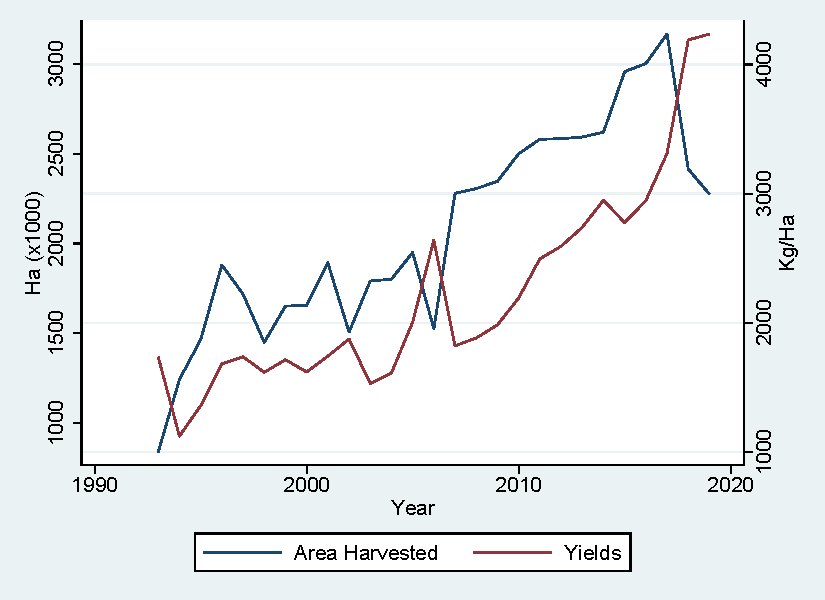
\includegraphics{results/figures/Maize_yields.pdf}
    \caption{Maize: Total area harvested and Average yields}
    \figcaption{Source: Authors' calculations using FAO stats data
    Note: Yield means the harvested production per ha for the area under cultivation}
    \label{fig:maize_yields}
\end{figure}


\section{Context}

Evidence has shown that the adoption of improved seed leads to increases in agricultural yields \citep{Carter2014-fm}, food security \citep{Shiferaw2014-op} and poverty reduction \citep{Minten2008-tj}. Despite such positive impacts, the low adoption levels of improved seeds varieties in Sub-Saharan Africa remains a puzzle. 


Multiple explanations have been proposed for observed adoption rates, including the type of technology promotion mechanisms used by governments, NGO’s, and businesses, the characteristics of the improved seeds and their adaptation to specific agro-climatic environments \citep{Bird2020-nt}, as well as growing conditions, such as the type of soil, input use, and other farmer characteristics \citep{Munshi2004-og}. The consensus in this literature is that the success of improved varieties depends on a range of factors that need to be better understood. Success of improved seeds should be accompanied by complementary conditions and inputs that would allow the full potential of these varieties to be realized. Specifically, extension services and on-farm field trials, seed variety characteristics and rainfall have been found to be crucial to the adoption of improved maize in Tanzania \citep{Kaliba2000-jh}. In the specific case of Ethiopia, labor, fertilizer use, farmers’ experience with extension packages, rainfall suitability and prices have been shown to increase the opportunity cost of not adopting improved wheat varieties \citep{Wale2006-bv}. Market access and the accessibility of extension services are also critical in the adoption of improved chickpea varieties in Ethiopia \citep{Verkaart2019-ol}. Other important determinants of heterogeneous effects include risk aversion \citep{Holden2016-vy}, farm size \citep{Ghimire2015-bd}, and credit constraints \citep{Simtowe2008-jn,Balana2020-hx}.



A different branch of the literature provides an alternative explanation for such low adoption rates, focusing on heterogeneous potential returns to adoption \citep{Suri2011-oi}. This literature suggests that even if returns to adoption are high, farmers may fail to adopt if they face low comparative advantage to adoption. Other methods used in the literature fail to account for this heterogeneity, admitting only the presence of time-constant and/or time-varying unobserved heterogeneities (depending on the data structure) for identification purposes \citep{Kassie2018-xn,Falco2011-rt}. These methods ignore the possibility of a farmer’s comparative advantage of using an improved technology over a traditional one as playing a central role in their adoption decision. 


We rely on Suri’s method and its extension in \citep{Tjernstrom_Emilia_Dalia_Ghanem_Oscar_Barriga_Cabanillas_Travis_J_Lybbert_Jeffrey_D_Michler_and_Aleksandr_Michuda2020-bc} to account for such heterogeneous comparative advantages and evaluate how these are explained by climatic conditions. In Ethiopia, rainfall deviations from historical averages are found to be the main driver of heterogeneous effects for adopting agronomic packages \citep{Marenya2020-kb}. Similar experiences from Malawi show exposure to past droughts is found to increase the adoption of drought-tolerant maize among farmers that also receive subsidies \citep{Katengeza2019-af} and the dis-adoption of traditional local maize \citep{Holden2016-vy}.

We will contribute to this literature by considering historical climate averages on the suitability of improved varieties to understand whether adoption is indeed realized where its potential is highest. Moreover, we will contribute to the understanding of how water conservation innovations and irrigation mitigate the effects of droughts on the potential of improved seeds.



\section{Data}

The current study uses the Ethiopia Socioeconomic Survey (ESS), a part of the Agricultural Sample Survey (AgSS), a survey designed to obtain production estimates for the major crops. The survey is a join effort of the the Central Statistics Agency of Ethiopia, the World Bank and CGIAR (Consortium of International Agricultural Research Centers) \citep{kosmowski2020shining} that aims at collecting information from a representative sample of households in the  the most populous regions of the country. The ESS contains several questionnaires targeted at getting an understanding of the state of agriculture. This includes a survey that is conducted post-planting and then post-harvest. These surveys are more important to our analysis as it gives a close look to inputs used in agriculture, the types of seeds used (in various levels of detail) and yields collected post-harvest.

There were significant differences between the analysis carried out in ESS 1-3 and the most recent, ESS4. Most notably, the ESS4 is no longer a panel dataset made up of the households of ESS 1-3, but it includes important information on the DNA fingerprinting of seed type, with which we can calculate misclassification rates. This is important information as the first three waves of ESS only included self-reported hybrid maize status. Since our estimation strategy requires a balanced panel dataset of maize growers, our main analysis will include the first three waves of the ESS. We use the fourth wave later for validation, and to explore the impact of specific types of improved seeds.

Figure \ref{map:regions} shows the spatial distribution of the locations of the our households of study. As previously mentioned these are households that grow either improved or conventional maize and that are observed for all three rounds of the survey. Most households come from the northwest region of Amhara, Tigray and Oromiya which is consistent with where maize is mostly grown in Ethiopia \citep{Abate2015-rj}.

\begin{figure}
    \centering
    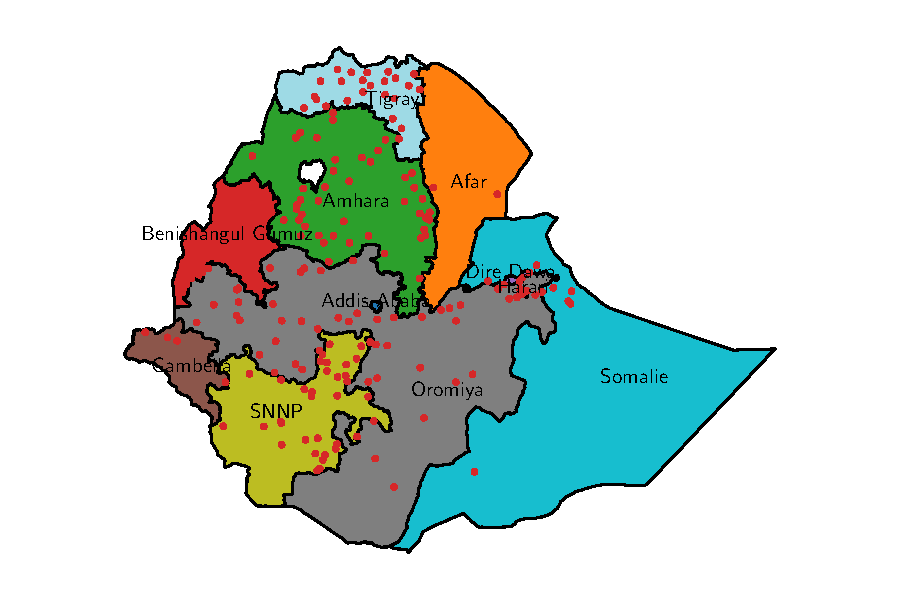
\includegraphics{results/figures/map_hhids.pdf}
    \caption{Spatial Distribution of Households Surveyed}
    \figcaption{Note: Green markers denote the locations of households}
    \label{map:regions}
\end{figure}

Table \ref{tbl:summary} shows a set of summary statistics for our sample. The mean parcel size for a household is about 0.15 Ha, with a maximum size of a little less than 1.5 Ha. Harvest labor is disproportionately skewed to family participation with around 20 days of harvest labor being conducted by family members and only about 2 days for hired labor. This is indicative of either malfunctioning labor markets, income constraints or high supervision costs. The distances to some key areas are also highlighted in Table \ref{tbl:summary}. On average households are around 13 kilometers away from an asphalt road and almost 60 kilometers away from the nearest market. This makes both the purchase of improved seed and the marketing of yields subject to transportation costs and a difficult enterprise. Fertilizer costs are on average 8,350 Birr (~178 USD) and with a large amount of the sample not using fertilizer at all. This is particularly important in the context of improved maize seed use as it requires fertilizer to be most effective. Only 5\% of the sample irrigates their crops making households susceptible weather shocks.

% \resizebox{0.7\textwidth}{!}{
{\small\tabcolsep=3pt  % hold it local
    \begin{table}
\centering
\caption{Summary Statistics for Households}
\label{tbl:summary}
\begin{tabular}{lllll}
\toprule
                             & Wave &       1.0 &       2.0 &       3.0 \\
\midrule
Parcel Size & N &  1,116.00 &  1,116.00 &  1,116.00 \\
                             & Mean &      0.31 &      0.32 &      0.30 \\
                             & Std. Dev. &      0.36 &      0.39 &      0.35 \\
Household Labor for Harvest (Days) & N &  1,116.00 &  1,116.00 &  1,116.00 \\
                             & Mean &     45.51 &     38.29 &     36.33 \\
                             & Std. Dev. &     71.11 &     54.58 &     46.56 \\
Hired Labor for Harvest (Days) & N &  1,116.00 &  1,116.00 &  1,116.00 \\
                             & Mean &      4.27 &      3.38 &      4.89 \\
                             & Std. Dev. &     25.93 &     17.08 &     54.11 \\
Age of Household Head & N &  1,106.00 &  1,086.00 &  1,102.00 \\
                             & Mean &     43.85 &     45.91 &     48.23 \\
                             & Std. Dev. &     14.31 &     14.17 &     14.33 \\
Sex of Household Head & N &  1,109.00 &  1,114.00 &  1,108.00 \\
                             & Mean &      1.15 &      1.15 &      1.16 \\
                             & Std. Dev. &      0.36 &      0.36 &      0.36 \\
Years of Education of Household Head & N &  1,106.00 &  1,085.00 &  1,102.00 \\
                             & Mean &      1.46 &      1.56 &      1.64 \\
                             & Std. Dev. &      2.71 &      2.77 &      2.92 \\
Total Rainfall (mm) & N &  1,113.00 &  1,088.00 &  1,106.00 \\
                             & Mean &    899.23 &    953.98 &    943.03 \\
                             & Std. Dev. &    240.43 &    237.46 &    267.07 \\
Does Household have Title to land? & N &  1,113.00 &  1,088.00 &  1,106.00 \\
                             & Mean &      0.43 &      0.52 &      0.61 \\
                             & Std. Dev. &      0.50 &      0.50 &      0.49 \\
Crop Cut Dry Yield (kg/ha) & N &  1,105.00 &  1,103.00 &  1,103.00 \\
                             & Mean &     86.51 &    251.69 &    438.42 \\
                             & Std. Dev. &    200.25 &    532.17 &    786.49 \\
Self-reported Yields (kg/ha) & N &  1,043.00 &  1,075.00 &  1,064.00 \\
                             & Mean &    187.18 &  1,314.04 &  1,224.65 \\
                             & Std. Dev. &    435.03 &  1,157.66 &  1,105.53 \\
\bottomrule
\multicolumn{6}{l}{Note: Parcel size, yield and distance variables winsorized at the 1\% level.}
\end{tabular}
\end{table}

}

The ESS has has both self-reported and crop cut yields available. This provides two sources of yield information, although self-reported yields seem to be overly large compared to either fresh or dried crop cut yields. Self-reported yields are both more susceptible to behavioral biases, but also to confusion caused by differences in assumed units. In general, though, the sample with available yield information cuts down the available sample immensely, which limits the power of the estimation. It isn't clear whether unavailable yields numbers is due to some sort of selection or whether crop cuts were only collected randomly from a few households.

\subsection{Improved seeds}

Defining what constitutes an improved seed is challenging because of the different characteristics of seeds. A crop seed is considered “improved” in Ethiopia if it was tested by breeders and evaluated to be superior to existing varieties (MoA, 2013, SPIA, 2020). In Ethiopia, the government controls most of the seed system. Local agricultural offices or extension agents assess the demands of different varieties, the MoA decides the seed quantities to be produced, and actors such as regional seed enterprises, seed companies, seed unions, are involved in the production of certified seeds; and seeds are primarily distributed by seed producer cooperatives (SPCs), which account for 37\% of total distribution in the country (SPIA, 2020). 

An improved seed can be obtained directly from such distribution centers (which would distribute a first generation seed), or it could be cultivated from second or posterior generations from the originally bred seed. Farmers are asked to report whether the variety they used was a first-generation improved seed, second generation,  recycled, or a traditional variety. When buying seeds, farmers might be able to identify the variety they are looking for, but it is unlikely that they would be aware of the source. 

Fifty four varieties have been released in Ethiopia since 1990, out of which seven were released between 1990 to 1999, 29 between 2000 to 2009, and 18 between 2010 to 2019. Thirty four of such varieties contain CIMMYT germplasm, out of which, 10 Drought-tolerant maize varieties (DTMZ) and 8 Quality protein maize (QPM) were released (most of these between 2010 to 2019). Out of the CIMMYT-related germplasm, ten are Open-pollinated varieties (OPVs) and 25 are hybrid. 
The fourth wave of the ESS introduced for the first time DNA fingerprinting for barley, maize, and sorghum. The collection of crop-cuts for crop yield estimation facilitated the process for DNA fingerprinting. For the crop-cuts, a 4 square meter quadrant was randomly selected in each plot, so that total production harvested from such patch was weighted (both when freshly harvested and when dried). The DNA material was extracted from samples from such dried crop-cuts, that were then matched with the genetic material of the maize DNA reference library for Ethiopia, obtained from a CIMMYT and EIAR project. The collection of DNA samples focused only on eight regions. In each EA of such regions, a random sample of plots was selected, of a maximum of 10 fields for each crop. As a result, 505 plots were selected for DNA fingerprinting, which corresponded to 447 households. 

The DNA fingerprinting process matched the genetic material of each sampled harvest with that of the reference library. The resulting matching process returns the name of the crop variety matched, its germplasm origin or their pedigree (whether they are a CIMMYT line, EIAR, IITA or private), the breeder or maintainer, and the year of their release (which could be indicative of the number of generations a seed had been cultivated), as well as the genetic purity of the sample (the degree of no contamination by other genetic varieties). It also informs whether the harvested seeds are open-pollinated varieties (OPVs) or hybrids; drought-tolerant maize varieties (DMTZ) or quality protein maize (QPM). This rich information about seed varieties provides a unique opportunity to further understand impacts differentiated by type of seed, degree of purity, year of release or source. Figure \ref{fig:adoption_r4} shows adoption rates in the fourth round for improved varieties, using the above characteristics as different definitions.

We find that 38\% of households self-report adopting a “new” improved variety (SR2 in Figure \ref{fig:adoption_r4}), and 43\% report adopting a “new”, “second generation” or “recycled” improved variety (SR1). Considering a household as adopter if the household planted an improved variety in at least one of their plots, all households where a DNA sample was obtained used a maize improved seed, considering a purity threshold of 70\% (DNA 70). When purity thresholds of 90 and 95\% are considered (DNA 90, DNA 95 in Figure \ref{fig:adoption_r4}, respectively), adoption rates change to 91 and 54\% of households, respectively. 62\% of households adopted a High-yielding variety, compared to 38\% that adopted an open-pollinated variety, and 15\% of households adopted a Drought-tolerant maize variety. 63\% of households that adopted an improved variety are using a CGIAR-derived germplasm, and 79\% are using an exotic germplasm. Finally, 64\% of households adopted a variety that was released on the year 2000 or after, and 24\% adopted a variety that was adopted in the year 2010 or after.

\begin{figure}
    \centering
    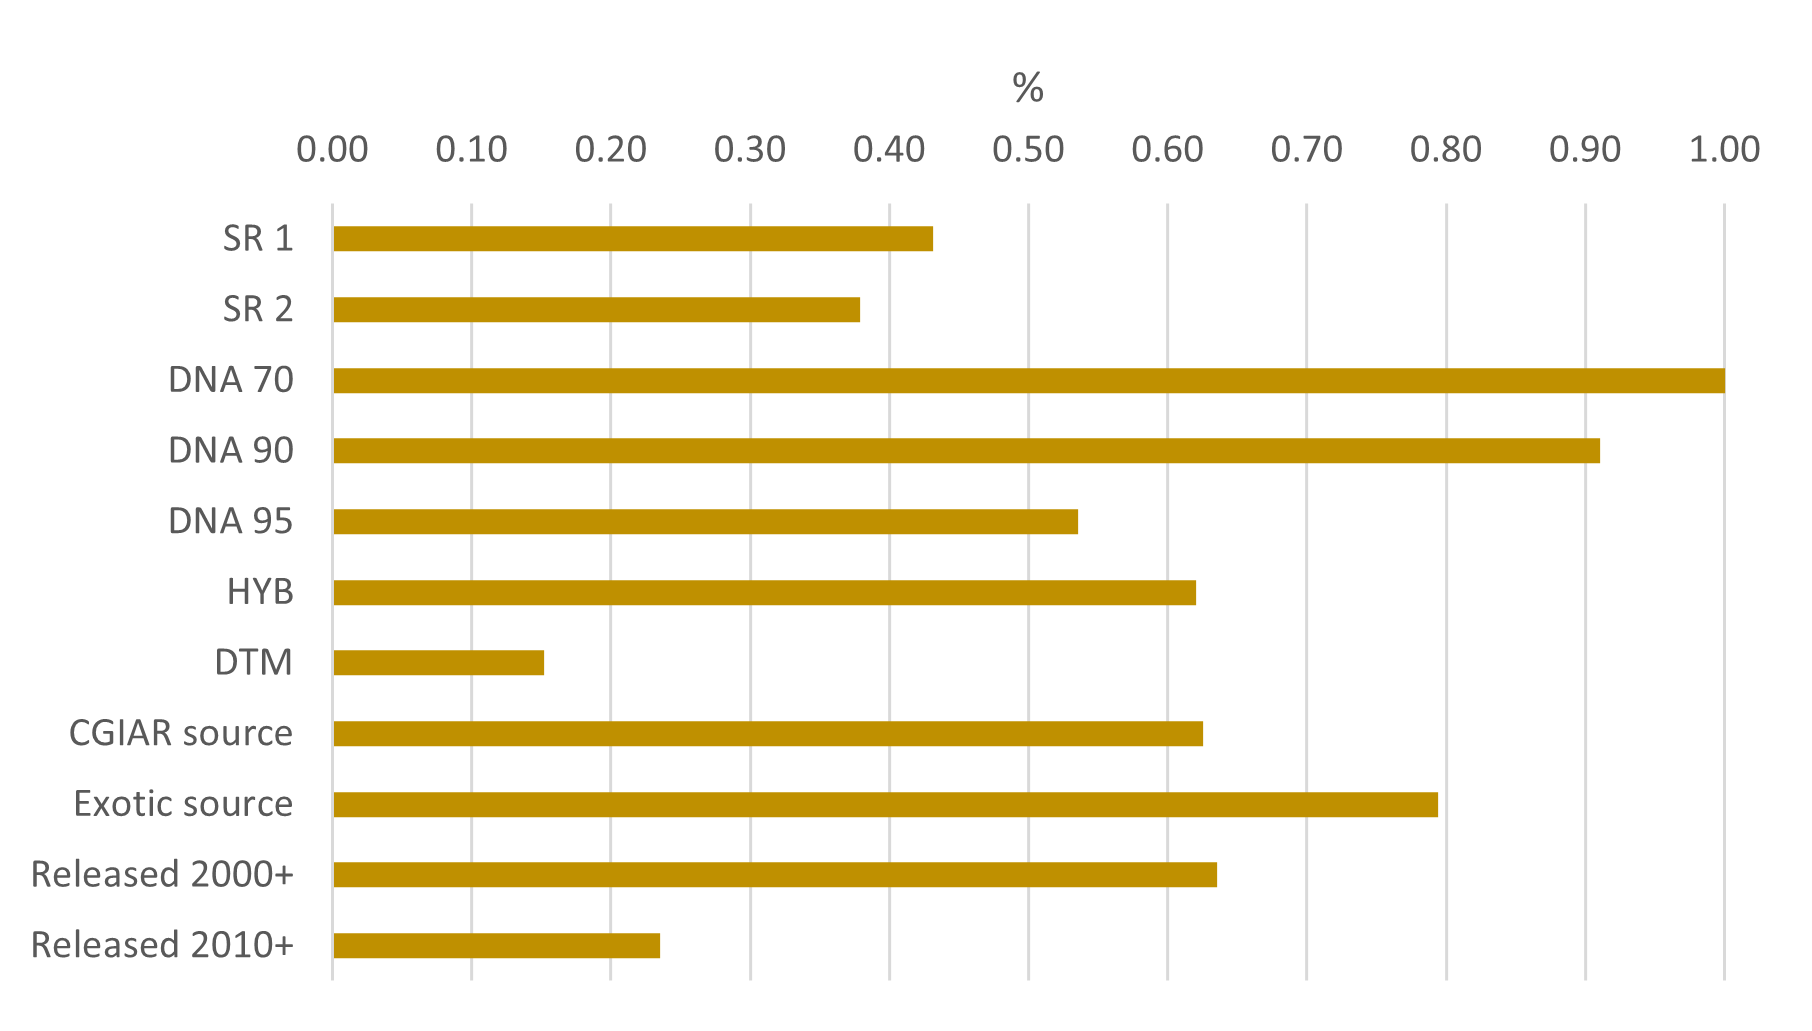
\includegraphics{results/figures/adoption_r4.png}
    \caption{Adoption rates of improved varieties in 2018 (by self-report, purity level, crop type, source and year of release)}
    \figcaption{Note: Shares represent the proportion of adopters among maize farmers. Acronyms include: SR1 [=1 if New, 2nd gen or recycled, =0 if Traditional]; SR2  [=1 if New, =0 if 2nd gen, recycled or traditional]; DNA70 - Improved if purity $>=$70$\%$; DNA90 - Improved if purity $>=$90$\%$; DNA95 - Improved if purity $>=$95$\%$; HYB - Improved DNA, [=1 Hybrid, 0=Open pollinated]; DTM - Drought tolerant Maize [=1 DTM, 0=otherwise], CGIAR source [=1 if germplasm associated to a CGIAR-related thread], Exotic source [=1 if germplasm associated to an exotic source], Released 2000+ [=1 if DNA associated to a variety released on year 2000 or later], Released 2010+ [=1 if DNA associated to a variety released on year 2010 or later]. QPM is not included as there are too few households planting QPM seeds (n=6).}
    \label{fig:adoption_r4}
\end{figure}

These ratios are in line with prior findings. In the regions of Oromia, Amhara, Tigray, and SNNPR, adoption rates of improved maize varieties of 39\% of households were found, according to self-reported information (Zeng et al., 2015). In the regions of Amhara, Benishangul-Gumuz, Oromia, SNNPR, and Tigray, adoption rates of improved maize varieties were found for 27\% of households (Jaleta et al., 2018). In Oromia, SNNPR, and Benishangul-Gumuz adoption of improved varieties per farmers’ self-reports was found for 84\% of maize growers in 2011, and 88\% of maize growers in 2013 (Yirga et al., 2017).

Understanding the effects of improved seed adoption is not only challenging because there could be multiple ways of establishing what constitutes an improved seed, but also because such definitions may or may note overlap, or because farmers may also missclassify a variety as improved. Figure \ref{fig:missclassification} shows the correlation between the different definitions discussed above. For those seeds for which genetic material was obtained, the correlation with the self-reported seeds indicator is low, especially when using lower cutoff thresholds. 

\begin{figure}
    \centering
    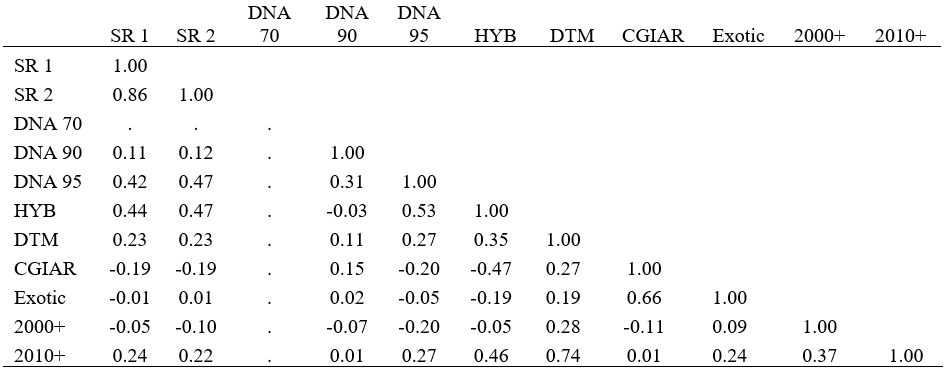
\includegraphics{results/figures/missclassification.png}
    \caption{Correlation of different definitions of improved seeds, 4th round}
    \figcaption{Note: Shares represent the proportion of adopters among maize farmers. Acronyms include: SR1 [=1 if New, 2nd gen or recycled, =0 if Traditional]; SR2  [=1 if New, =0 if 2nd gen, recycled or traditional]; DNA70 - Improved if purity $>=$70$\%$; DNA90 - Improved if purity $>=$90$\%$; DNA95 - Improved if purity $>=$95$\%$; HYB - Improved DNA, [=1 Hybrid, 0=Open pollinated]; DTM - Drought tolerant Maize [=1 DTM, 0=otherwise], CGIAR source [=1 if germplasm associated to a CGIAR-related thread], Exotic source [=1 if germplasm associated to an exotic source], Released 2000+ [=1 if DNA associated to a variety released on year 2000 or later], Released 2010+ [=1 if DNA associated to a variety released on year 2010 or later]. QPM is not included as there are too few households planting QPM seeds (n=6).}
    \label{fig:missclassification}
\end{figure}

\section{Estimation Strategy}

\subsection{Group Random Coefficient Model}

The advantage of our estimation strategy is that we do not rely on identification from a valid instrument, but modelling the heterogeneity directly through a projection of their returns to adoption on their observed "trajectory" of adoption. This allows us to directly capture two effects: the heterogeneous effects of the so-called "comparative advantage" of adoption, and, under the assumption of linearity in comparative advantage, a description of the overall economy's sorting of farmers based on their comparative advantage. The first is important because it is able to disentangle the effect of a general household's agricultural ability (which can be thought of as a fixed effect) and their adoption-specific potential. The sorting parameter can tell us whether the economy sorts such that those that would benefit the most adoption actually adopt, or whether there are barriers that stop that sorting from happening. See \cite{Tjernstrom_Emilia_Dalia_Ghanem_Oscar_Barriga_Cabanillas_Travis_J_Lybbert_Jeffrey_D_Michler_and_Aleksandr_Michuda2020-bc} for more information on the assumptions involved for the Group Random Coefficients estimator. In our particular case, we contribute to the literature and methodology of \cite{Tjernstrom_Emilia_Dalia_Ghanem_Oscar_Barriga_Cabanillas_Travis_J_Lybbert_Jeffrey_D_Michler_and_Aleksandr_Michuda2020-bc} by providing reasonable ways to aggregate the results of the GRC model, which may seem difficult to interpret in its raw form. We use these aggregations to better understand how adoption affects households across time, as well as whether the frequency of adoption has a strong effect.

\begin{table}
\centering
\caption{Trajectories of Households}
\label{tbl:trajectories}
\begin{tabular}{lrr}
\toprule
Trajectory &  Frequency &    Share \\
\midrule
       000 &       2124 & 0.611927 \\
       111 &        456 & 0.131374 \\
       011 &        228 & 0.065687 \\
       001 &        219 & 0.063094 \\
       010 &        153 & 0.044080 \\
       100 &        108 & 0.031115 \\
       110 &         96 & 0.027658 \\
       101 &         87 & 0.025065 \\
\bottomrule
\multicolumn{3}{l}{Note: Table shows frequency and shares of each trajectory in sample. 1 denotes adoption and 0 otherwise. The first digit is for whether the household adopted in wave 1, the second digit for wave and the third digit for wave 3}
\end{tabular}
\end{table}


Table \ref{tbl:Trajectories} maps out the frequencies of the different trajectories present in the data, sorted by frequency. The largest portion of the data are those that do not adopt improved maize seed at all, followed with sharp decline, to those that use improved maize seed in every period. Interestingly, adoption trajectories seem to be more popular for later adoptions than earlier ones. Most households do not adopt at all (``never-adopters''), but the second most frequent trajectory are those that adopt in every wave (``always-adopters''). Let $\mathcal{H}$ be the set of these trajectories in the data and let $\mathcal{H}_S$ be the set of switcher trajectories, i.e. $\mathcal{H}_S = \mathcal{H}\backslash\{(0,0,0), (1,1,1)\}$

To generate results for adoption, we use the unrestricted model as outlined in \cite{Tjernstrom_Emilia_Dalia_Ghanem_Oscar_Barriga_Cabanillas_Travis_J_Lybbert_Jeffrey_D_Michler_and_Aleksandr_Michuda2020-bc}:

\begin{align}
y_{it}&=\sum_{\underline{h}\in\mathcal{H}\backslash (1,1,1)}\mu_{\underline{h}}+\sum_{\underline{h}\in\mathcal{H}_{S}}\Delta_{\underline{h}}h_{it}1\{h_{i}=\underline{h}\} + \kappa_{(1,1,1)}h_{it}1\{\underline{h}=(1,1,1)\}+ X_{it}\beta+\varepsilon_{it}.\label{eq:GRC}
\end{align}

where $y$ is log yields, $\mu_{\underline{h}}$ are binary variables for being in trajectory $\underline{h}$, $h$ is a binary variable for whether household $i$ adopted in wave $t$, $X$ are a set of controls and $\Delta_{0,0,1}$ are the returns to adoption for trajectory $(0,0,1)$. $\kappa_{(1,1,1)}$ is the average yield with adoption of the always-adopters, where $\kappa_{(1,1,1)} = \mu_{(1,1,1)} + \Delta_{(1,1,1)}$. It is not possible to separately identify $\mu_{(1,1,1)}$ and $\Delta_{(1,1,1)}$ without adding more structure to the model in the form of the linearity in comparative advantage (LCA) restriction, which we explain how to test for below.


We estimate comparative advantage using the restricted model:

\begin{align}
y_{it}&=\sum_{\underline{h}\in\mathcal{H}\backslash (1,1,1)}\mu_{\underline{h}}+\Delta_{(0,0,1)}h_{it}+\phi(\mu_{(0,0,1)}-\mu_{(0,0,1)})h_{it}1\{h_{i}=(0,0,1)\}\nonumber\\
&~~~+\left(\mu_{(1,1,1)}+\phi\left(\mu_{(1,1,1)}-\mu_{(0,0,1)}\right)\right)h_{it}1\{h_{i}=(1,1,1)\} + X_{it}\beta +\varepsilon_{it},\label{eq:GRC_Suri}
\end{align}

where $\phi$ is the parameter which describes sorting in the economy. If $\phi$ is positive, then higher yields is associated with higher comparative advantage, denoting that those that adopt also tend to have the highest returns to adoption. If it is negative, however, this denotes that there might be barriers, such as a lack of fertilizer access, and bad roads that restrict the ability to buy hybrid seed. $\phi$ is estimated in two ways: through the restricted model just mentioned and by a weak-identification brute force grid procedure, which allows for calculating the confidence interval for $\phi$ for multiple sets of trajectories. The advantage of the weak-identification robust procedure is that we can test for whether the data satisfies the conditions necessary for an interpretable $\phi$ parameter.

Equation \ref{eq:GRC_Suri} can be estimated by way of General Method of Moments. Parameters for returns to adoption and comparative advantage can be post-estimated by the delta method, where the expression for returns of each trajectory can be derived from:

$$
\Delta_{\underline{h}}=\phi\left(\mu_{\underline{h}}-\mu_{(0,0,1)}\right) + \Delta_{(0,0,1)}
$$

for trajectory $\underline{h} \neq (0,0,1)$.\footnote{Since we use $(0,0,1)$ as our base, we already have returns available for that trajectory, namely $\Delta_{(0,0,1)}$} Comparative advantage can be derived from:

$$
\theta_{\underline{h}} = \mu_{\underline{h}} - E(\mu_{\underline{h}})
$$

where $E(\mu_{\underline{h}}) = \sum_{\mathcal{H}} \pi_h \cdot \mu_h$ for $\pi_h$ being the frequency weight for trajectory $h$. The comparative advantage of each trajectory tells us how much a household with a given trajectory benefits from adoption. $\theta <0 $ denotes that returns to adoption are negative and that a household loses by adopting.

Once we generate $\theta$ and $\Delta$ for each trajectory, we can examine heterogeneous effects to adoption. In its raw form, that means that have eight comparative advantages available for comparison, which is rich in its information, but difficult to interpret as a result, we will aggregate $\theta$ in two ways to improve interpretability: (1) which wave the household adopted, and (2) the number of time adoption took place. We do this by taking a simple average, grouped by each of these factors.

\subsection{Endogenous Switching regression}
The ESS4 is a unique data-set that includes DNA fingerprinting of maize seed type. This brings new possibilities in terms of exploring.... sayESS4 no longer part of panel but that still useful,.... \par
The group random coefficient model used the variation in the adoption trajectories of each observation in the ESS 1-3 panel as a source of information that allows for an unbiased estimation. ESS4 is no longer part of this panel data-set, hence, in order to estimate the effect of the adoption of improved seeds on yields, an alternative estimation method is needed. We propose an endogenous switching regression model which accounts for unobserved heterogeneity in adoption decisions. This method imposes restrictive assumptions regarding the distribution of the errors of the selection and output equations. At the same time, the exclusion restriction needs to be satisfied in order to reduce the bias of the estimation. Nevertheless, the endogenous switching regression holds certain advantages over other methodologies used for identifying unbiased estimates with cross-sectional observational data such as propensity score matching or other instrumental variable approaches (\cite{shiferaw2014adoption}) and has been used to study similar questions in the past (\citealt{falco2011does}, \citealt{kabunga2012yield}). \par
The decision to adopt and improved seed is determined by a series of observed and unobserved variables. Equation \ref{eq:switch_latent} shows the definition for a latent variable $A^*$ that reflects the benefit from adopting an improved seed relative to planting a traditional one. As shown in the equation, household $i$ will decide to adopt  (A_i=1). 

\begin{align}
A_i^*=Z_i\alpha+\varepsilon_i \; \text{with} \, A_i    \begin{cases}
      1, & \text{if}\ A_i^*>0 \\
      0, & \text{otherwise}
    \end{cases} \label{eq:switch_latent}
\end{align}


\section{Results}

\subsection{Group Random Coefficients}

Our results use two definitions of yields: measured cropcuts of dry maize and self-reported yields maize yields. Each measure of yields has its benefits and drawbacks. Cropcuts, for instance, provides a true estimate of yields for a given parcel of land, but it is at the cost of a reduced sample size. Self-reports have larger sample sizes, but may suffer from measurement error. For controls we use the years of education of the household head, the age of the household head, the sex of the household head, whether there is a title for the land being cultivated, the parcel size in hectares, as well as the hours of household and hired labor. Commensurate with the literature, we also include interactions of these controls with hybrid adoption as added controls. The results of the regression are shown in Table \ref{tbl:unres}.

% {\small\tabcolsep=3pt  % hold it local
\resizebox{1\textwidth}{!}{
{
\def\sym#1{\ifmmode^{#1}\else\(^{#1}\)\fi}
\begin{tabular}{l*{3}{c}}
\hline\hline
          &\multicolumn{1}{c}{(1)}&\multicolumn{1}{c}{(2)}&\multicolumn{1}{c}{(3)}\\
          &\multicolumn{1}{c}{Log Dry Cropcuts}&\multicolumn{1}{c}{Log Dry Cropcuts}&\multicolumn{1}{c}{Log Dry Cropcuts}\\
\hline
$\mu_{000}$&    6.350\sym{***}&    1.075\sym{***}&    5.849\sym{***}\\
          & (0.0372)         &  (0.132)         &  (0.202)         \\
$\mu_{001}$&    6.246\sym{***}&    0.720\sym{***}&    5.771\sym{***}\\
          &  (0.121)         &  (0.209)         &  (0.231)         \\
$\mu_{010}$&    6.405\sym{***}&    1.166\sym{***}&    6.049\sym{***}\\
          &  (0.151)         &  (0.301)         &  (0.259)         \\
$\mu_{011}$&    5.518\sym{***}&    0.218         &    5.324\sym{***}\\
          &  (0.207)         &  (0.496)         &  (0.310)         \\
$\mu_{100}$&    6.479\sym{***}&    1.002\sym{***}&    5.798\sym{***}\\
          &  (0.145)         &  (0.270)         &  (0.254)         \\
$\mu_{101}$&    6.466\sym{***}&    0.347         &    5.654\sym{***}\\
          &  (0.193)         &  (0.407)         &  (0.309)         \\
$\mu_{110}$&    6.908\sym{***}&    1.546\sym{***}&    6.271\sym{***}\\
          &  (0.277)         &  (0.401)         &  (0.335)         \\
$\Delta_{001}$&    0.634\sym{***}&    1.067\sym{***}&   -5.395\sym{***}\\
          &  (0.241)         &  (0.330)         &  (0.322)         \\
$\Delta_{010}$&   0.0398         &   -0.964\sym{**} &   -6.405\sym{***}\\
          &  (0.318)         &  (0.461)         &  (0.403)         \\
$\Delta_{011}$&    1.308\sym{***}&    1.137\sym{**} &   -5.100\sym{***}\\
          &  (0.249)         &  (0.519)         &  (0.342)         \\
$\Delta_{100}$&   -0.699\sym{***}&   -0.984\sym{**} &   -6.364\sym{***}\\
          &  (0.252)         &  (0.389)         &  (0.294)         \\
$\Delta_{101}$&    0.112         &    1.183\sym{***}&   -5.381\sym{***}\\
          &  (0.321)         &  (0.422)         &  (0.388)         \\
$\Delta_{110}$&   -0.302         &   0.0558         &   -6.376\sym{***}\\
          &  (0.304)         &  (0.395)         &  (0.354)         \\
\hline
Observations&      984         &      930         &      930         \\
Controls  &       No         &      Yes         &      Yes         \\
Interact w/ Hybrid&       No         &       No         &      Yes         \\
\hline\hline
\multicolumn{4}{l}{\footnotesize Standard errors in parentheses}\\
\multicolumn{4}{l}{\footnotesize \sym{*} \(p<0.10\), \sym{**} \(p<0.05\), \sym{***} \(p<0.01\)}\\
\end{tabular}
}

}

\resizebox{1\textwidth}{!}{
\centering
% \begin{tabular}{l*{6}{c}}}
\toprule
{} &           Base &      Controls & Controls w/ Int. \\
\midrule
Restriction 001-010 &      (-$\infty$, $\infty$) &     (-$\infty$, $\infty$) &        (-$\infty$, $\infty$)	&      (-$\infty$, $\infty$) &  (-3.37, -1.33) &      (-$\infty$, -.49)  	\\
Restriction 001-011 &   (-1.81, .01) &     (-$\infty$, $\infty$) &        (-$\infty$, $\infty$) 			&      (-$\infty$, $\infty$) &       (-$\infty$, $\infty$) &        (-$\infty$, $\infty$) \\
Restriction 001-100 &      (-$\infty$, $\infty$) &     (-$\infty$, $\infty$) &        (-$\infty$, $\infty$)	&      (-$\infty$, $\infty$) &       (-$\infty$, $\infty$) &        (-$\infty$, $\infty$) \\
Restriction 001-101 &      (-$\infty$, $\infty$) &     (-$\infty$, $\infty$) &        (-$\infty$, $\infty$)	&    (-1.34, $\infty$) &       (-$\infty$, $\infty$) &        (-$\infty$, $\infty$) \\
Restriction 001-110 &  (-7.11, -.49) &   (-$\infty$, -.02) &        (-$\infty$, $\infty$) 					&  (-3.37, -.56) &    (-$\infty$, -1.27) &   (-5.84, -1.07) \\
\hline\\Joint Test  &         $\emptyset$ &  (-$\infty$, -2.32) &     (-$\infty$, -1.92) 					&         $\emptyset$ &  (-4.91, -1.34) &     (-$\infty$, -1.95) \\
\bottomrule
\end{tabular}

\begin{tabular}{llll}
\toprule
{} &           Base &        Controls & Controls w/ Int. \\
\midrule
Restriction 001-010 &      (-$\infty$, $\infty$) &  (-3.37, -1.33) &      (-$\infty$, -.49) \\
Restriction 001-011 &      (-$\infty$, $\infty$) &       (-$\infty$, $\infty$) &        (-$\infty$, $\infty$) \\
Restriction 001-100 &      (-$\infty$, $\infty$) &       (-$\infty$, $\infty$) &        (-$\infty$, $\infty$) \\
Restriction 001-101 &    (-1.34, $\infty$) &       (-$\infty$, $\infty$) &        (-$\infty$, $\infty$) \\
Restriction 001-110 &  (-3.37, -.56) &    (-$\infty$, -1.27) &   (-5.84, -1.07) \\
\hline\\Joint Test  &         $\emptyset$ &  (-4.91, -1.34) &     (-$\infty$, -1.95) \\
\bottomrule
\end{tabular}

\begin{tabular}{llll}
\toprule
{} &           Base &      Controls & Controls w/ Int. \\
\midrule
Restriction 001-010 &      (-$\infty$, $\infty$) &     (-$\infty$, $\infty$) &        (-$\infty$, $\infty$) \\
Restriction 001-011 &   (-1.81, .01) &     (-$\infty$, $\infty$) &        (-$\infty$, $\infty$) \\
Restriction 001-100 &      (-$\infty$, $\infty$) &     (-$\infty$, $\infty$) &        (-$\infty$, $\infty$) \\
Restriction 001-101 &      (-$\infty$, $\infty$) &     (-$\infty$, $\infty$) &        (-$\infty$, $\infty$) \\
Restriction 001-110 &  (-7.11, -.49) &   (-$\infty$, -.02) &        (-$\infty$, $\infty$) \\
\hline\\Joint Test  &         $\emptyset$ &  (-$\infty$, -2.32) &     (-$\infty$, -1.92) \\
\bottomrule
\end{tabular}

}
% {
\def\sym#1{\ifmmode^{#1}\else\(^{#1}\)\fi}
\begin{tabular}{l*{3}{c}}
\hline\hline
          &\multicolumn{1}{c}{(1)}&\multicolumn{1}{c}{(2)}&\multicolumn{1}{c}{(3)}\\
          &\multicolumn{1}{c}{Log Dry Cropcuts}&\multicolumn{1}{c}{Log Dry Cropcuts}&\multicolumn{1}{c}{Log Dry Cropcuts}\\
\hline
$\mu_{000}$&    6.587\sym{***}&    1.110\sym{***}&    6.444\sym{***}\\
          & (0.0310)         &  (0.144)         &  (0.134)         \\
$\mu_{001}$&    6.659\sym{***}&    1.261\sym{***}&    6.622\sym{***}\\
          &  (0.103)         &  (0.198)         &  (0.159)         \\
$\mu_{010}$&    6.942\sym{***}&    1.177\sym{***}&    6.835\sym{***}\\
          &  (0.118)         &  (0.229)         &  (0.186)         \\
$\mu_{011}$&    5.968\sym{***}&    0.518         &    5.930\sym{***}\\
          &  (0.363)         &  (0.459)         &  (0.393)         \\
$\mu_{100}$&    6.759\sym{***}&    1.551\sym{***}&    6.685\sym{***}\\
          &  (0.114)         &  (0.248)         &  (0.173)         \\
$\mu_{101}$&    7.011\sym{***}&    1.292\sym{***}&    6.838\sym{***}\\
          &  (0.166)         &  (0.327)         &  (0.213)         \\
$\mu_{110}$&    7.120\sym{***}&    1.520\sym{***}&    6.983\sym{***}\\
          &  (0.124)         &  (0.289)         &  (0.180)         \\
$\Delta_{001}$&    0.209         &   -0.180         &   -7.050\sym{***}\\
          &  (0.152)         &  (0.182)         &  (0.202)         \\
$\Delta_{010}$&   0.0531         &    0.191         &   -7.174\sym{***}\\
          &  (0.138)         &  (0.163)         &  (0.207)         \\
$\Delta_{011}$&    1.241\sym{***}&    1.024\sym{**} &   -6.002\sym{***}\\
          &  (0.380)         &  (0.468)         &  (0.412)         \\
$\Delta_{100}$&    0.718\sym{***}&    0.678         &   -6.484\sym{***}\\
          &  (0.136)         &  (0.572)         &  (0.205)         \\
$\Delta_{101}$&    0.157         &   -0.214         &   -6.984\sym{***}\\
          &  (0.262)         &  (0.342)         &  (0.299)         \\
$\Delta_{110}$&   -0.421\sym{***}&   -0.281         &   -7.497\sym{***}\\
          &  (0.158)         &  (0.189)         &  (0.233)         \\
\hline
Observations&     2320         &     2289         &     2289         \\
Controls  &       No         &      Yes         &      Yes         \\
Interact w/ Hybrid&       No         &       No         &      Yes         \\
\hline\hline
\multicolumn{4}{l}{\footnotesize Standard errors in parentheses}\\
\multicolumn{4}{l}{\footnotesize \sym{*} \(p<0.10\), \sym{**} \(p<0.05\), \sym{***} \(p<0.01\)}\\
\end{tabular}
}


\begin{figure}
    \centering
    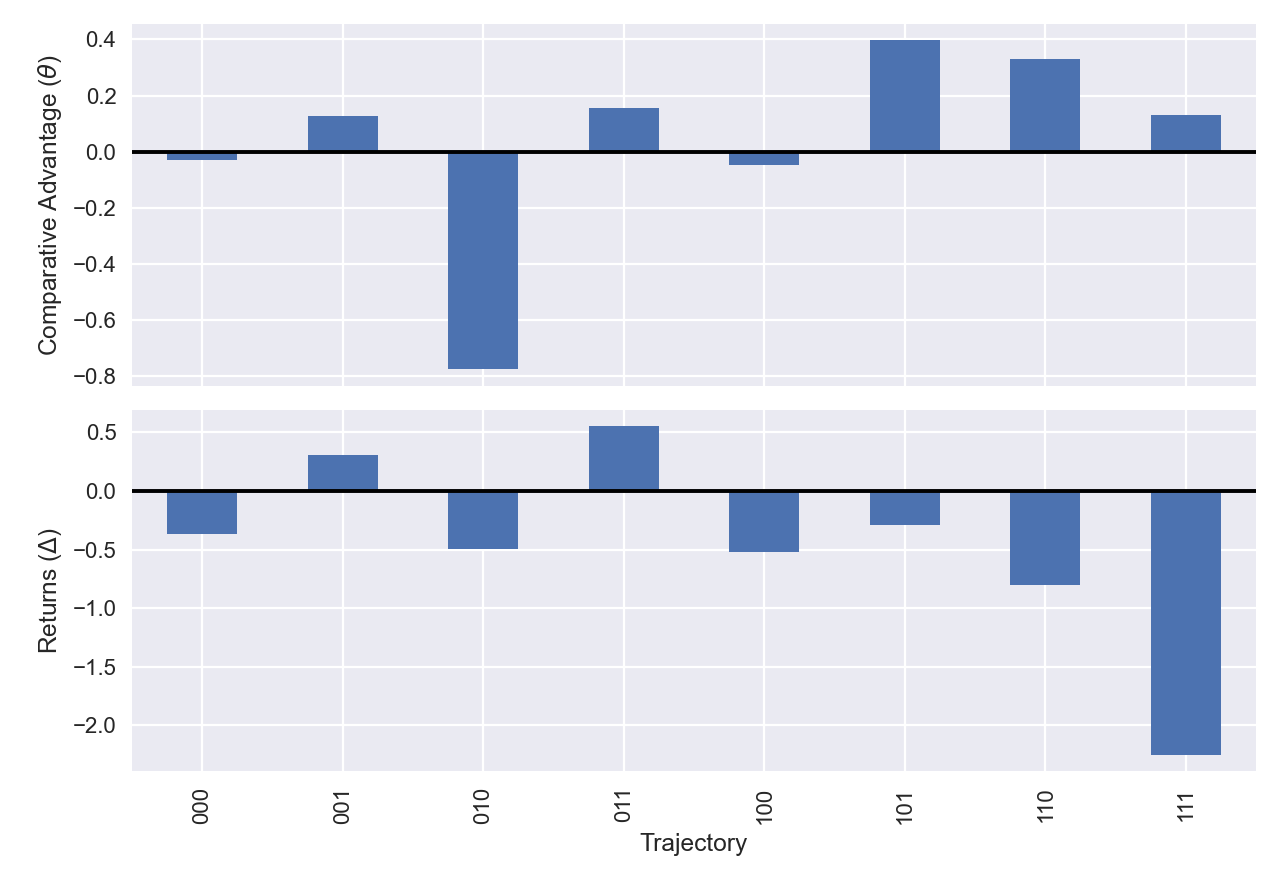
\includegraphics[scale=0.75]{results/figures/theta.png}
    \caption{Comparative Advantage and Returns by Trajectory (Dry Cropcuts)}
    \label{fig:theta_delta_raw}
\end{figure}

\begin{figure}
    \centering
    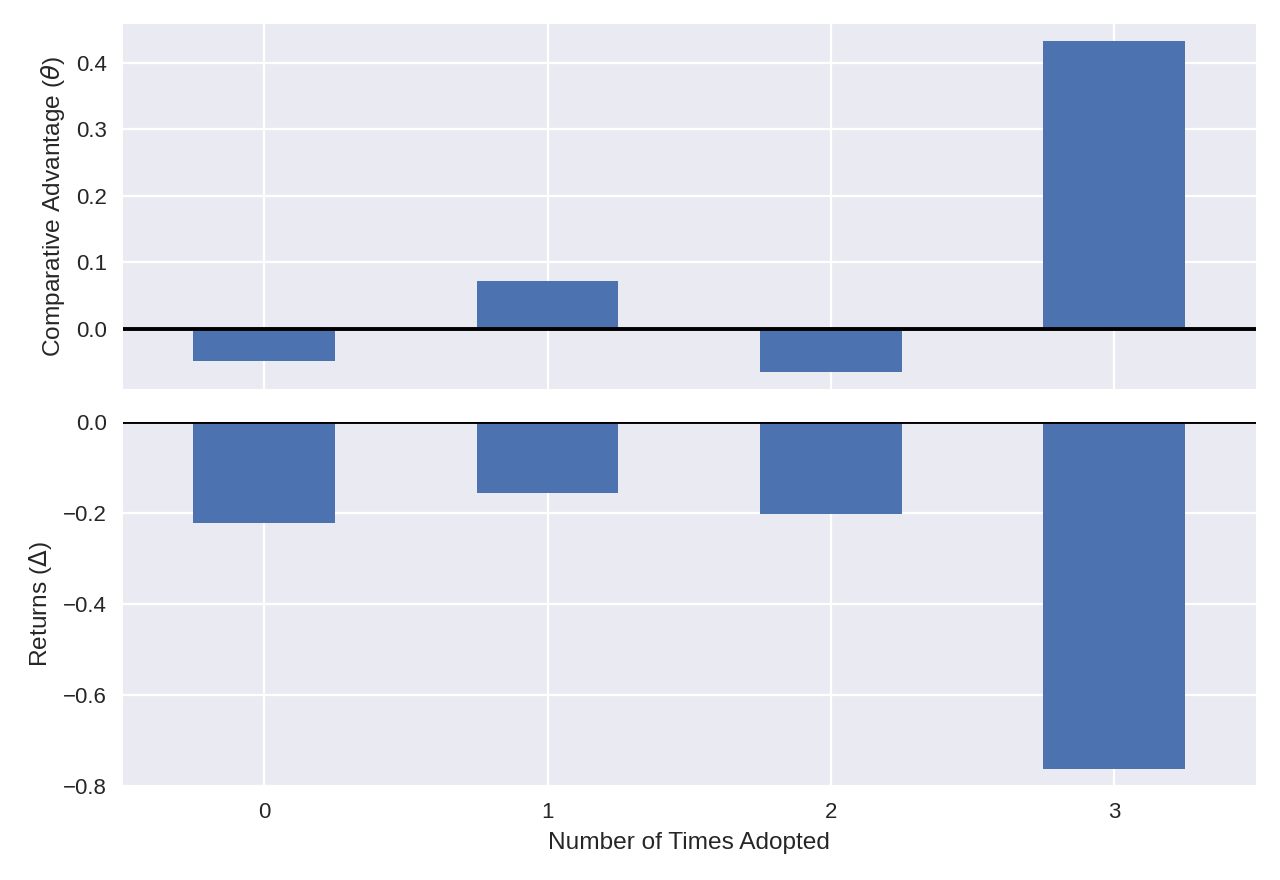
\includegraphics[scale=0.75]{results/figures/traj_sum.png}
    \caption{Aggregation Results: Comparative Advantage and Returns by the Number of Times Adopted (Dry Cropcuts}
    \label{fig:traj_sum}
\end{figure}

\begin{figure}
    \centering
    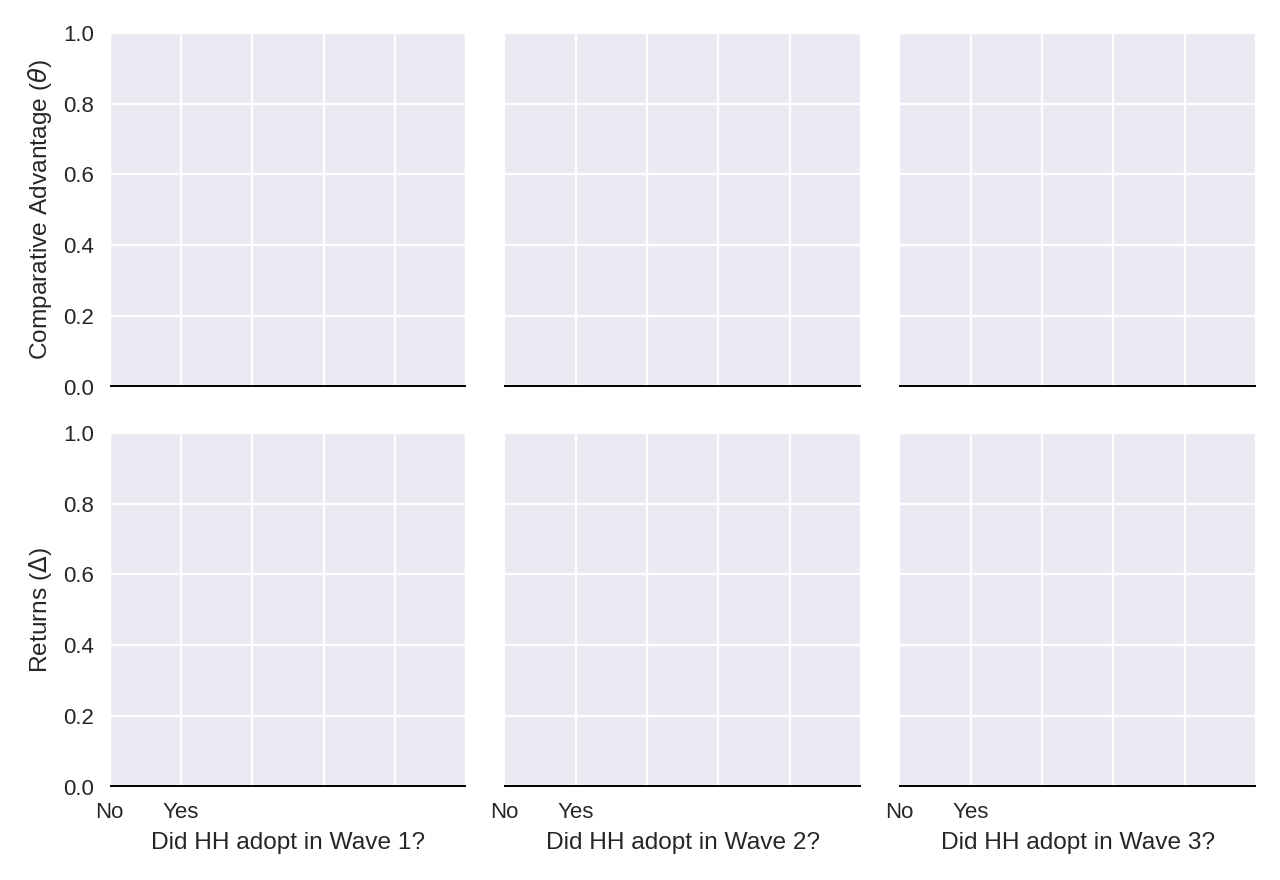
\includegraphics[scale=0.75]{results/figures/when_adopt_cropcut.png}
    \caption{Aggregation Results: Comparative Advantage and Returns by Wave of Adoption (Dry Cropcuts}
    \label{fig:when_adopt}
\end{figure}

\subsection{Endogenous Switching Regression}

We first examine the results of the Endogenous Switching Regression using a self-reported definition of an improved variety. As before, we consider a more loose definition of improved variety, which includes new seeds but also second-generation and recycled (SR1), and a more strict definition, which includes only new varieties (SR2). Table \ref{tab:switch1} shows the results of the Switching regression using both definitions, and using self-reported and cropcut yields. We see that regardless of the definition of improved seed, yields measurement form and types of controls included, the results consistently show that the Average Treatment effect on the Treated (ATT) is negative and the Average Treatment effect on the Untreated (ATU) is positive, meaning that farmers that adopted a self-reported improved seed would've been better off not adopting, and farmers that did not adopt a self-reported improved seed would've been better off adopting. 

\begin{table}[H]
\centering
\hspace*{-1.2cm}
\begin{threeparttable}
\caption{Effects on yields (log) from adopting improved maize varieties (self-reported)}
\label{tab:switch1}
\begin{tabular}{l cccccc}
\hline
\hline
            &Adopters yields&Non-adopters yields&         ATE&          SE&     p-value\\
\hline
\textit{SR1, SR yields}&            &            &            &            &            \\
ATT         &        7.30&        9.07&       -1.76&       0.011&      0.0000\\
%
%
%
ATU         &        9.06&        6.87&        2.19&       0.024&      0.0000\\
%
%
%
\textit{SR1, cropcut yields}&            &            &            &            &            \\
ATT         &        7.57&        7.86&       -0.30&       0.017&      0.0000\\
%
%
%
ATU         &        8.89&        7.11&        1.78&       0.039&      0.0000\\
%
%
%
\textit{SR1, SR yields, full set of controls}&            &            &            &            &            \\
ATT         &        7.28&        7.82&       -0.54&       0.019&      0.0000\\
%
%
%
ATU         &        9.65&        6.85&        2.80&       0.100&      0.0000\\
%
%
%
\textit{SR1, cropcut yields, full set of controls}&            &            &            &            &            \\
ATT         &        7.56&        7.61&      -0.049&       0.019&      0.0087\\
%
%
%
ATU         &        9.24&        7.11&        2.13&       0.085&      0.0000\\
%
%
%
\textit{SR2, SR yields}&            &            &            &            &            \\
ATT         &        7.30&        7.85&       -0.55&       0.020&      0.0000\\
%
%
%
ATU         &        9.63&        6.88&        2.75&       0.101&      0.0000\\
%
%
%
\textit{SR2, cropcut yields}&            &            &            &            &            \\
ATT         &        7.61&        7.62&      -0.013&       0.019&        0.47\\
%
%
%
ATU         &        9.35&        7.14&        2.21&       0.091&    1.6e-130\\
\hline
\hline
\end{tabular}
\begin{tablenotes}
\footnotesize
\item{Note: Full set of controls include: parcel size (in HA), household labor, hired labor, fertilizer costs, other input costs irrigation (dummy), mechanization (dummy), organic fertilizer (dummy). Instruments for the adoption equation include: years of education of hh head, age of hh head, female head, land title, asset index, seed costs. Results for SR2 include full set of controls. SR1=1 if New, 2nd gen or recycled,=0 if Traditional; SR2=1 if New, =0 2nd gen, recycled or traditional}
\end{tablenotes}
\end{threeparttable}
\end{table}


To better understand the above puzzling results, we explore similar yield estimations using the different definitions of improved seeds from the DNA fingerprinting. We run similar switching regressions using different thresholds of DNA purity (70, 90 and 95\% purity), for hybrid seeds (compared with open-pollinated varieties), and for Drought-tolerant maize (DTMZ). Table \ref{tab:switch2} shows the results. 

Given that all the plots sampled for DNA fingerprinting showed a purity percent of 70\% or higher, we need a counter-factual to compare these purity thresholds with non-adopters. We therefore consider as non-adopters those that self-reported using a traditional variety. We are aware that given the universality of improved varieties with a 70\% threshold or higher and given the high rates of missclassification, the control group for a 70\% threshold is likely to be contaminated with a high share of false-positives. But we also know the results are biased downwards and that the control group for higher shares of purity will be less contaminated, which may provide an interesting comparison. 

Table \ref{tab:switch2} shows that the estimations for purity thresholds of 70 and 90\% show similar patterns as before: non-adopters would've been better off adopting and adopters would've been better off not adopting. But when improved seeds with a purity of 95\% or higher are compared with self-reported traditional varieties or lower purity than 95\%, the ATT becomes positive and the ATU is still positive but significantly decreases (and it is even negative when self-reported yields are used). Farmers that adopted a variety with a 95\% purity or greater had significantly greater yields than if they had not adopted, considering that this is even a lower boundary. 

We get similar results for DTMZ. Farmers that adopted DTMZ (as tracked by the DNA germplasm) did obtain greater yields than if they had not adopted. Again this result may be biased downwards because of possible false-positives among the control group. The results for the comparison between hybrid and open-pollinated varieties are not significant (when using self-reported yields).

\begin{table}[H]
\centering
\hspace*{-1.2cm}
\begin{threeparttable}
\caption{Effects on yields (log) from adopting improved maize varieties (DNA fingerprinting)}
\label{tab:switch2}
\begin{tabular}{l cccccc}
\hline
\hline
            &Adopters yields&Non-adopters yields&         ATE&          SE&     p-value\\
\hline
\textit{DNA 70, SR yields}&            &            &            &            &            \\
ATT         &        7.17&        7.31&       -0.14&       0.026&      0.0000\\
%
%
%
ATU         &        8.76&        6.76&        2.00&       0.036&      0.0000\\
%
%
%
\textit{DNA 70, cropcut yields}&            &            &            &            &            \\
ATT         &        7.28&        8.48&       -1.21&       0.041&      0.0000\\
%
%
%
ATU         &        8.55&        7.27&        1.28&       0.042&      0.0000\\
%
%
%
\textit{DNA 90, SR yields}&            &            &            &            &            \\
ATT         &        7.18&        9.07&       -1.90&       0.023&      0.0000\\
%
%
%
ATU         &        7.01&        6.80&        0.21&       0.022&      0.0000\\
%
%
%
\textit{DNA 90, cropcut yields}&            &            &            &            &            \\
ATT         &        7.30&        8.72&       -1.43&       0.028&      0.0000\\
%
%
%
ATU         &        9.32&        7.24&        2.09&       0.034&      0.0000\\
%
%
%
\textit{DNA 95, SR yields}&            &            &            &            &            \\
ATT         &        7.30&        7.08&        0.22&       0.036&      0.0000\\
%
%
%
ATU         &        6.87&        6.86&       0.018&       0.029&      0.5496\\
%
%
%
\textit{DNA 95, cropcut yields}&            &            &            &            &            \\
ATT         &        7.52&        7.39&        0.13&       0.018&      0.0000\\
%
%
%
ATU         &        7.38&        7.12&        0.26&       0.024&      0.0000\\
%
%
%
\textit{HYB, SR yields}&            &            &            &            &            \\
ATT         &        7.28&        7.25&       0.030&       0.028&      0.2892\\
%
%
%
ATU         &        7.06&        6.85&        0.21&       0.028&      0.0000\\
%
%
%
\textit{HYB, cropcut yields}&            &            &            &            &            \\
ATT         &        7.51&        7.55&      -0.038&       0.017&      0.0289\\
%
%
%
ATU         &        7.58&        7.03&        0.55&       0.021&      0.0000\\
%
%
%
\textit{DTMZ, SR yields}&            &            &            &            &            \\
ATT         &        7.42&        6.53&        0.89&       0.074&      0.0000\\
%
%
%
ATU         &        7.11&        7.02&       0.089&       0.022&      0.0001\\
%
%
%
\textit{DTMZ, cropcut yields}&            &            &            &            &            \\
ATT         &        7.56&        6.76&        0.81&       0.058&     3.5e-44\\
%
%
%
ATU         &        8.04&        7.27&        0.77&       0.028&    9.4e-167\\
\hline
\hline
\end{tabular}
\begin{tablenotes}
\footnotesize
\item{Note: Full set of controls include: parcel size (in HA), household labor, hired labor, fertilizer costs, other input costs irrigation (dummy), mechanization (dummy), organic fertilizer (dummy). Instruments for the adoption equation include: years of education of hh head, age of hh head, female head, land title, asset index, seed costs. All results include full set of controls. DNA 70, 90 and 95 refer to improved varieties defined by DNA finerprinting with purity levels of 70, 90 and 95\%, respectively. HYB equals 1 for a hybrid variety, 0 for an open-pollinated variety. DTMZ equals 1 for a Drought-tolerant maize variety}
\end{tablenotes}
\end{threeparttable}
\end{table}


To further disaggregate the results, we finally explore the source of the improved varieties (CGIAR or exotic) and the year of the seed release. We find positive effects for adopters of CGIAR-sourced varieties when using self-reported yields. The results seem to be contradictory when using cropcut yields, but we should consider these are different samples, as cropcuts were obtained in a subsample of plots. Exotic-sourced varieties also show positive yield effects for adopters; and a negative ATU, meaning non-adopters are also better off not adopting. Newly released-seed varieties do consistently show positive ATT, when using both self-reported and cropcut yields.

\begin{table}[H]
\centering
\resizebox{0.8\textwidth}{!}{
\hspace*{-1.2cm}
\begin{threeparttable}
\caption{Effects on yields (log) from adopting improved maize varieties (DNA fingerprinting)}
\label{tab:switch3}
\begin{tabular}{l cccccc}
\hline
\hline
            &Adopters yields&Non-adopters yields&         ATE&          SE&     p-value\\
\hline
\textit{CGIAR source, SR yields}&            &            &            &            &            \\
ATT         &        7.13&        6.71&        0.43&       0.033&      0.0000\\
%
%
%
ATU         &        9.19&        6.89&        2.31&       0.018&      0.0000\\
%
%
%
\textit{CGIAR source, cropcut yields}&            &            &            &            &            \\
ATT         &        7.23&        8.98&       -1.75&       0.040&      0.0000\\
%
%
%
ATU         &        7.51&        7.40&        0.11&       0.015&      0.0000\\
%
%
%
\textit{Exotic source, SR yields}&            &            &            &            &            \\
ATT         &        7.13&        6.65&        0.48&       0.022&      0.0000\\
%
%
%
ATU         &        6.83&        6.89&      -0.060&       0.021&      0.0047\\
%
%
%
\textit{Exotic source, cropcut yields}&            &            &            &            &            \\
ATT         &        7.28&        7.18&       0.098&       0.032&      0.0023\\
%
%
%
ATU         &        6.73&        7.33&       -0.60&       0.021&      0.0000\\
%
%
%
\textit{Year 2000+, SR yields}&            &            &            &            &            \\
ATT         &        7.26&        5.55&        1.71&       0.046&      0.0000\\
%
%
%
ATU         &        8.87&        6.93&        1.94&       0.041&      0.0000\\
%
%
%
\textit{Year 2000+, cropcut yields}&            &            &            &            &            \\
ATT         &        7.55&        7.27&        0.28&       0.024&      0.0000\\
%
%
%
ATU         &        8.52&        7.25&        1.27&       0.027&      0.0000\\
%
%
%
\textit{Year 2010+, SR yields}&            &            &            &            &            \\
ATT         &        7.44&        6.92&        0.53&       0.039&      0.0000\\
%
%
%
ATU         &        8.98&        6.91&        2.07&       0.056&      0.0000\\
%
%
%
\textit{Year 2010+, cropcut yields}&            &            &            &            &            \\
ATT         &        7.57&        6.97&        0.60&       0.035&     8.6e-65\\
%
%
%
ATU         &        8.72&        7.25&        1.47&       0.019&           0\\
\hline
\hline
\end{tabular}
\begin{tablenotes}[flushleft]
\footnotesize
\item{Note: Full set of controls include: parcel size (in HA), household labor, hired labor, fertilizer costs, other input costs irrigation (dummy), mechanization (dummy), organic fertilizer (dummy). Instruments for the adoption equation include: years of education of hh head, age of hh head, female head, land title, asset index, seed costs. All results include full set of controls. }
\end{tablenotes}
\end{threeparttable}
}
\end{table}



\section{Discussion and Implications}

- Why do we see that increasing purity leads to positive ATE
- may be due to improved seed being more effective, but doesnt tell the whole story
- barrier to purchasing the seed and associated inputs for poorer households, leading to reuse of seeds and being less effective


Our work has far-reaching policy implications. The adoption and impact of agricultural technologies is inherently heterogeneous. Our methodology incorporates that from the outset, allowing us to investigate whether synergies between seed adoption and water conservation strategies interact; a key component to understanding how investment into such projects translates to economic returns. Moreover, our research informs on not only the adoption but also dis-adoption decisions of technologies as well. In this sense, we provide valuable information to policymakers on how to better target seed marketing or infrastructure to help agricultural households improve their livelihoods


\section{Conclusion}


\bibliography{references}


\end{document}